%----------------------------------------------------------------------------
%----------------------------------------------------------------------------
\begin{figure}
\begin{center}
\leavevmode
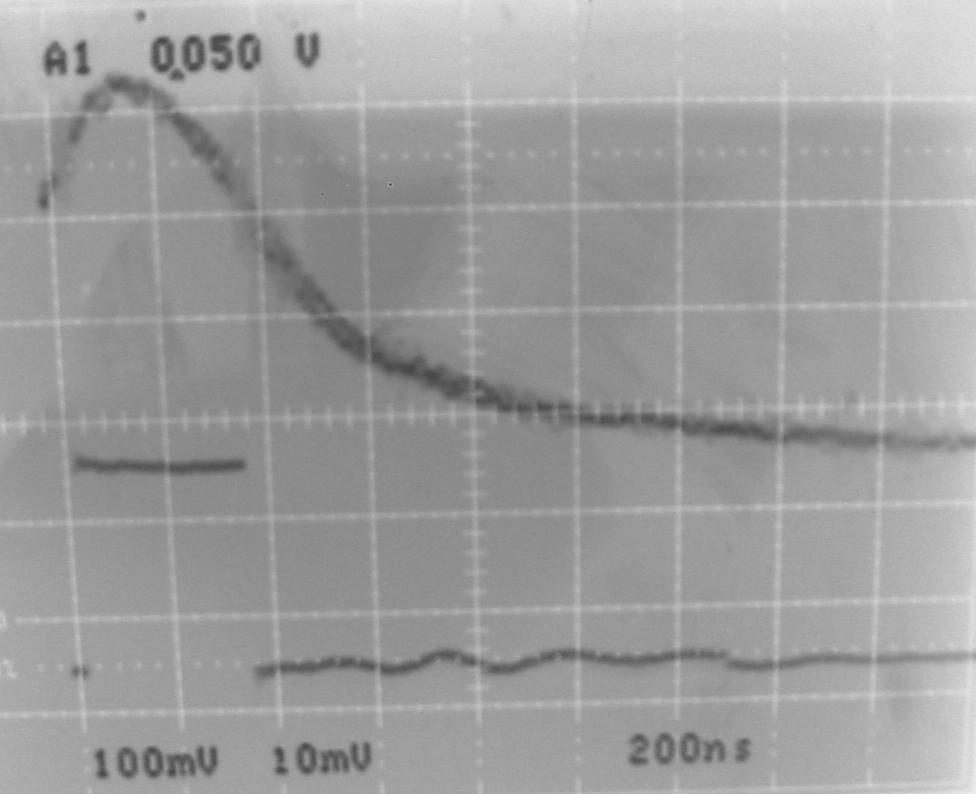
\includegraphics[width=4in]
{gate/gate.png}\\
\end{center}
\caption[Boxcar gate placement for RF beat measurement]{Boxcar gate placement for RF beat measurement. Channel one is the gate (lower trace, 100 mV/div), channel two is the receiver output (upper trace, 10 mV/div). This picture was taken with the receiver tuned to 50 MHz before we had the high pass filter, hence the large signal. Once the high pass filter was in place this ``DC'' signal was only $\sim$15 mV. This signal was only used to place the gate - data was not taken this close to DC.}
\label{gate}
\end{figure} 
%----------------------------------------------------------------------------
